%!TEX root = ../thesis.tex

\chapter{State of the Art}
\label{cha:stateofart}

In this chapter, we summarize the most relevant work on tracking, instance segmentation, and video object segmentation.
First, we focus on methods for tracking, and later, we talk about the state-of-the-art methods for instance segmentation and some implementations applied to videos.

\section{Tracking}
\label{sec:soa_tracking}

Tracking implementations are mainly focused on video object tracking.
This task consists in taking the bounding box surrounding an object and make bounding box predictions throughout the video that contains the object to track.

One state-of-the-art implementation is MDNet~\mdnet.
It proposes a Convolutional Neural Network with shared layers and multiple branches of domain-specific layers.
The architecture overview is showed at \figref{mdnet}.
Each branch is responsible for binary classification to identify the target in each specific video.
This domain-specific layers are updated online and the online tracking is performed by evaluating the candidate windows randomly sampled around the previous target state.
This method has led to state-of-the art results on tracking benchmarks and was the winner of the VOT Challenge~\votchallenge in 2016.

\begin{figure}[h]
  \centering
  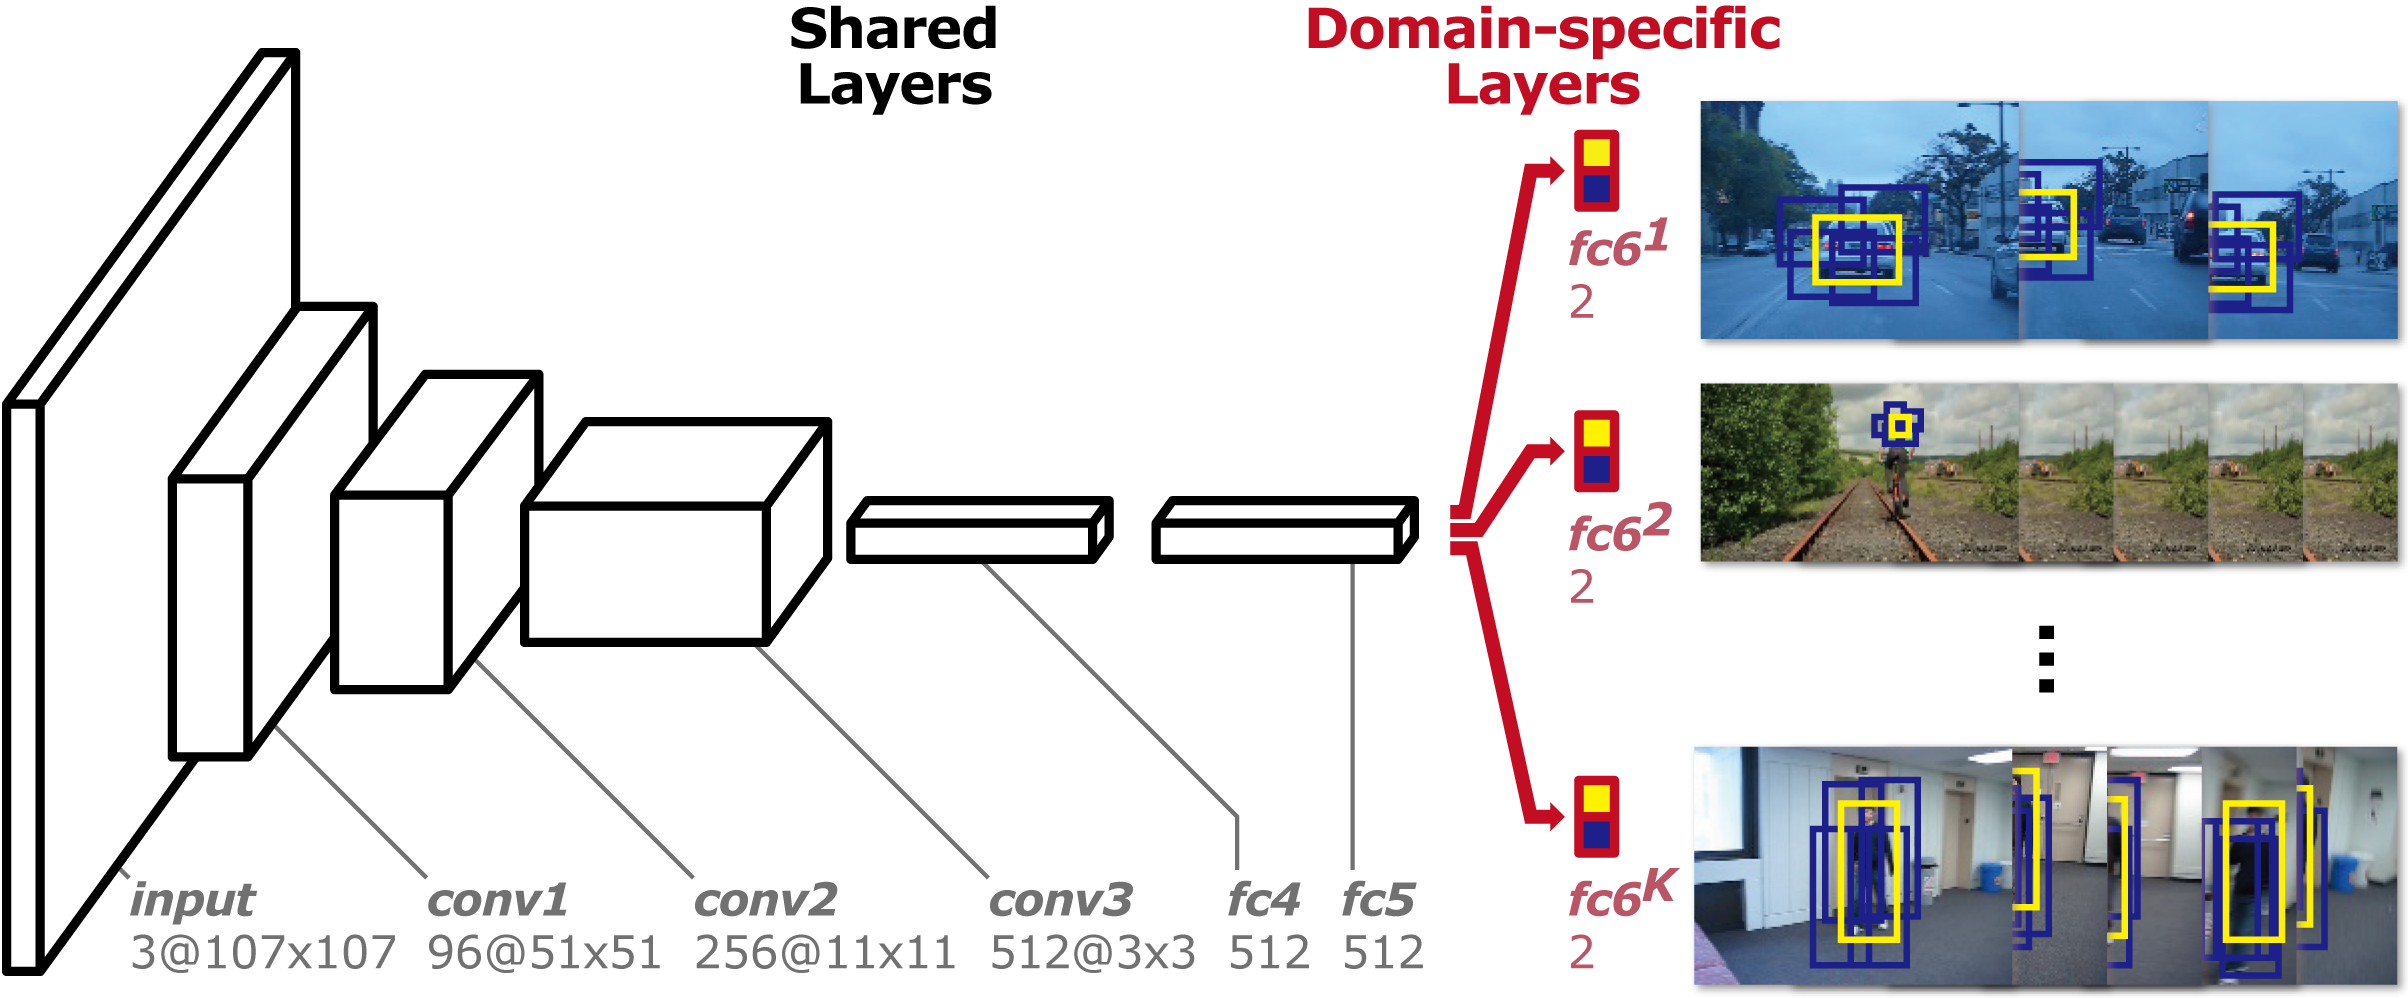
\includegraphics[width=.8\linewidth]{figures/mdnet/architecture.png}
  \caption{MDNet~\mdnet architecture. }
  \label{fig:mdnet}
\end{figure}

Different to MDNet, the idea behind this thesis focuses on keypoint tracking, rather than bounding boxes.

% Stacked Hourglass Networks for Human Pose Estimation~\cite{newell2016stacked}


\section{Semantic Instance Segmentation}
\label{sec:soa:instancesegmentation}

Semantic instance detection and segmentation is one of the most challenging tasks in Computer Vision right now.
In this section we explore some of the works that tackle instance segmentation in image domain. 

\paragraph{Mask R-CNN~\maskrcnn}
This work come from a series of works that started with object detection on images using Convolutional Neural Networks.\ToDo{Cite FastRCNN}
In a follow-up work, the same authors modify the architecture to make it differentiable, being able to train it end-to-end.\ToDo{Cite FasterRCNN}
Their most recent work, Mask R-CNN extends the same idea to predicting not only the bounding box of the detected object but its segmentation mask as well.
The idea behind this method consists of a CNN that with a forward pass extracts the features at the last convolutional layer.
Then a set of bounding box proposals are generated and the features in each proposed bounding box are used in one branch to predict a objectiveness score and bounding box regressions.
On this branch, a set of bounding boxes are obtained and score predicted. With these values, a second branch is responsible to predict a mask from each proposal.
The final prediction uses non-maximum suppression to reduce the number of the object proposals.
This approach shows state-of-the-art results on multiple datasets at the cost of using a very large amount (in the order of 1000s) proposals per image.
Some qualitative results can be found on \figref{maskrcnn}.

\begin{figure}[h]
  \centering
  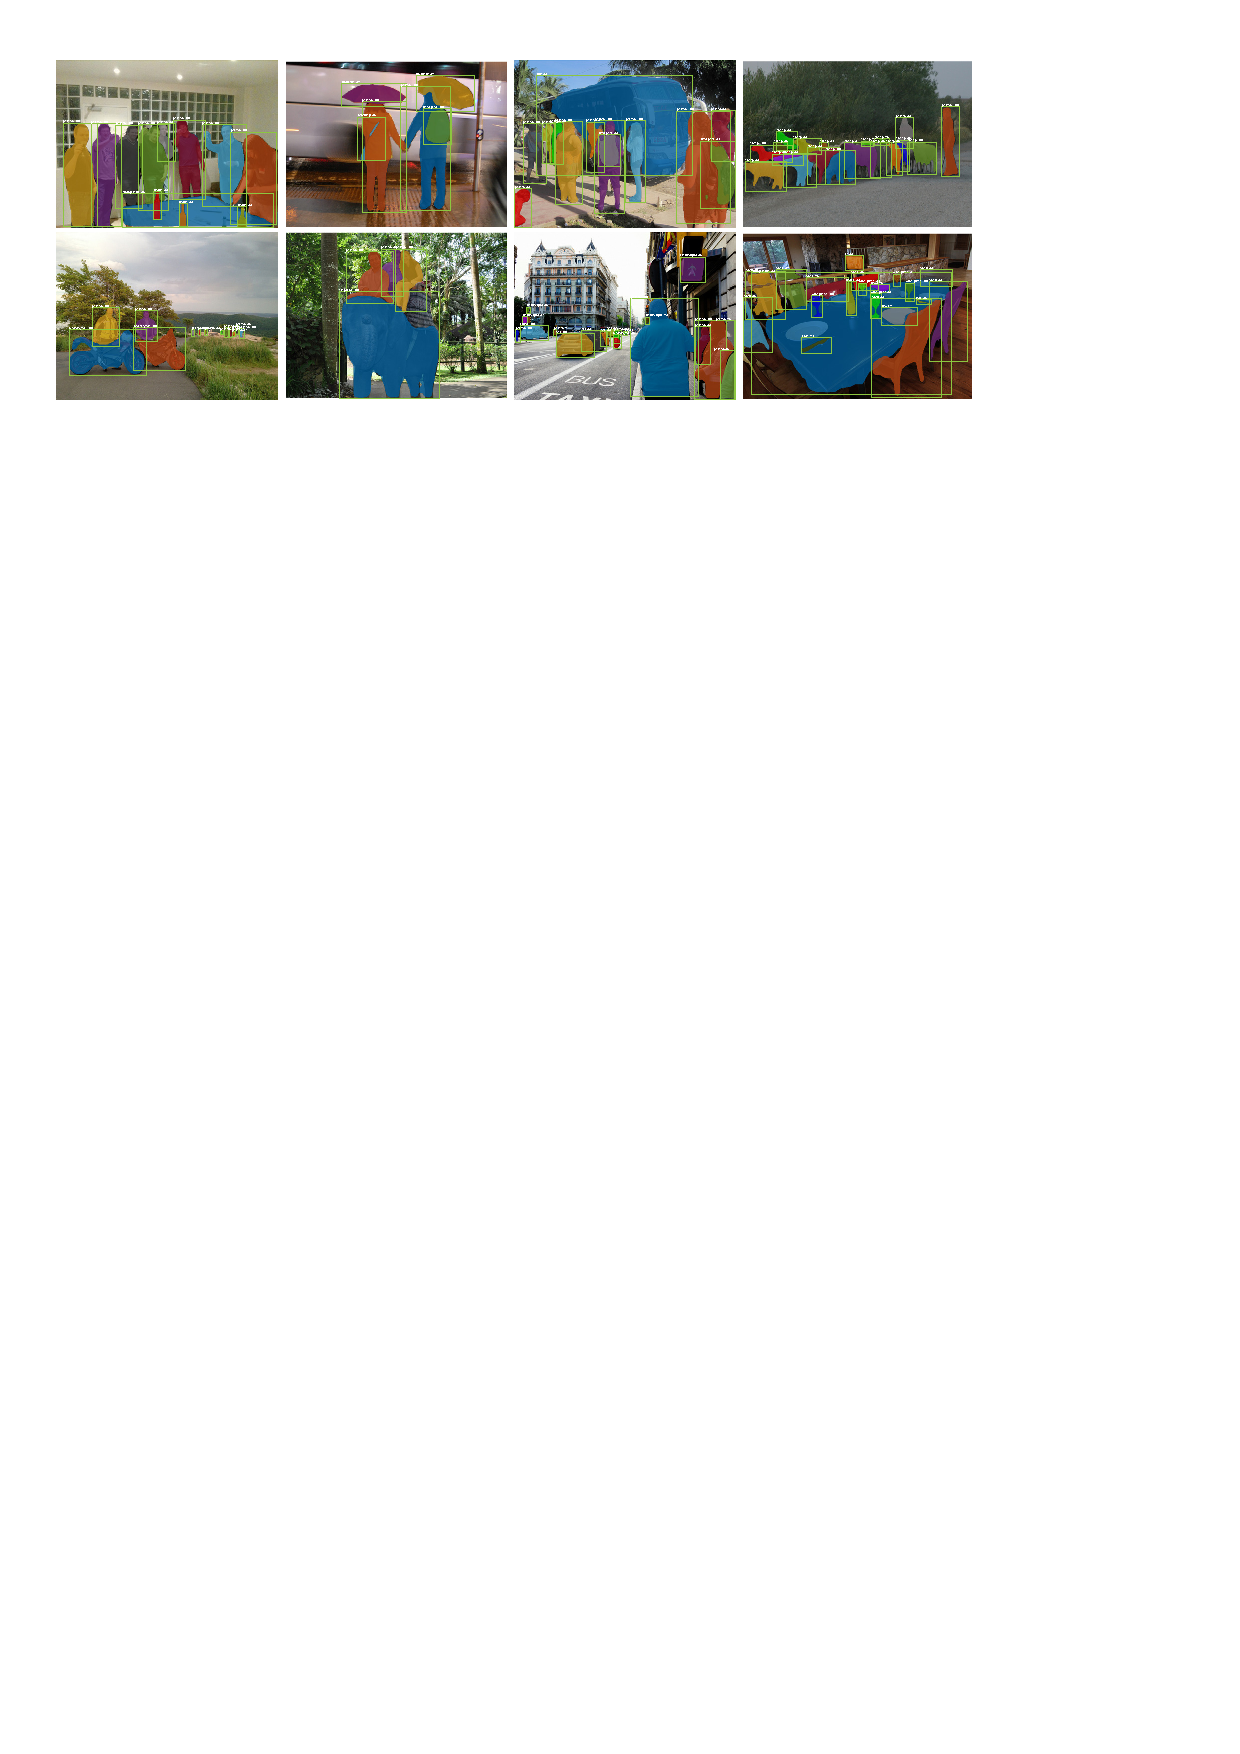
\includegraphics[width=1.\linewidth]{figures/maskrcnn/results.pdf}
  \caption{Mask R-CNN~\cite{he2017mask} results. }
  \label{fig:maskrcnn}
\end{figure}

\paragraph{Deep Metric Learning~\deepml}
This work also focuses on semantic instance segmentation on images.
They use a Convolutional Neural Network to predict an embedding representation per each pixel.
This network is trained using metric learning, regressing how likely two pixels are to belong to the same object.
Then they propose the use of seed points and its pairwise similarity to predict the instances and its masks on an image once the embedding for each pixels is computed.
Some results of the segmentations can be found on \figref{deep_metric_learning}.\ToDo{Link this work to your thesis (We also use deep metric.. to blabla..)}

\begin{figure}[h]
  \centering
  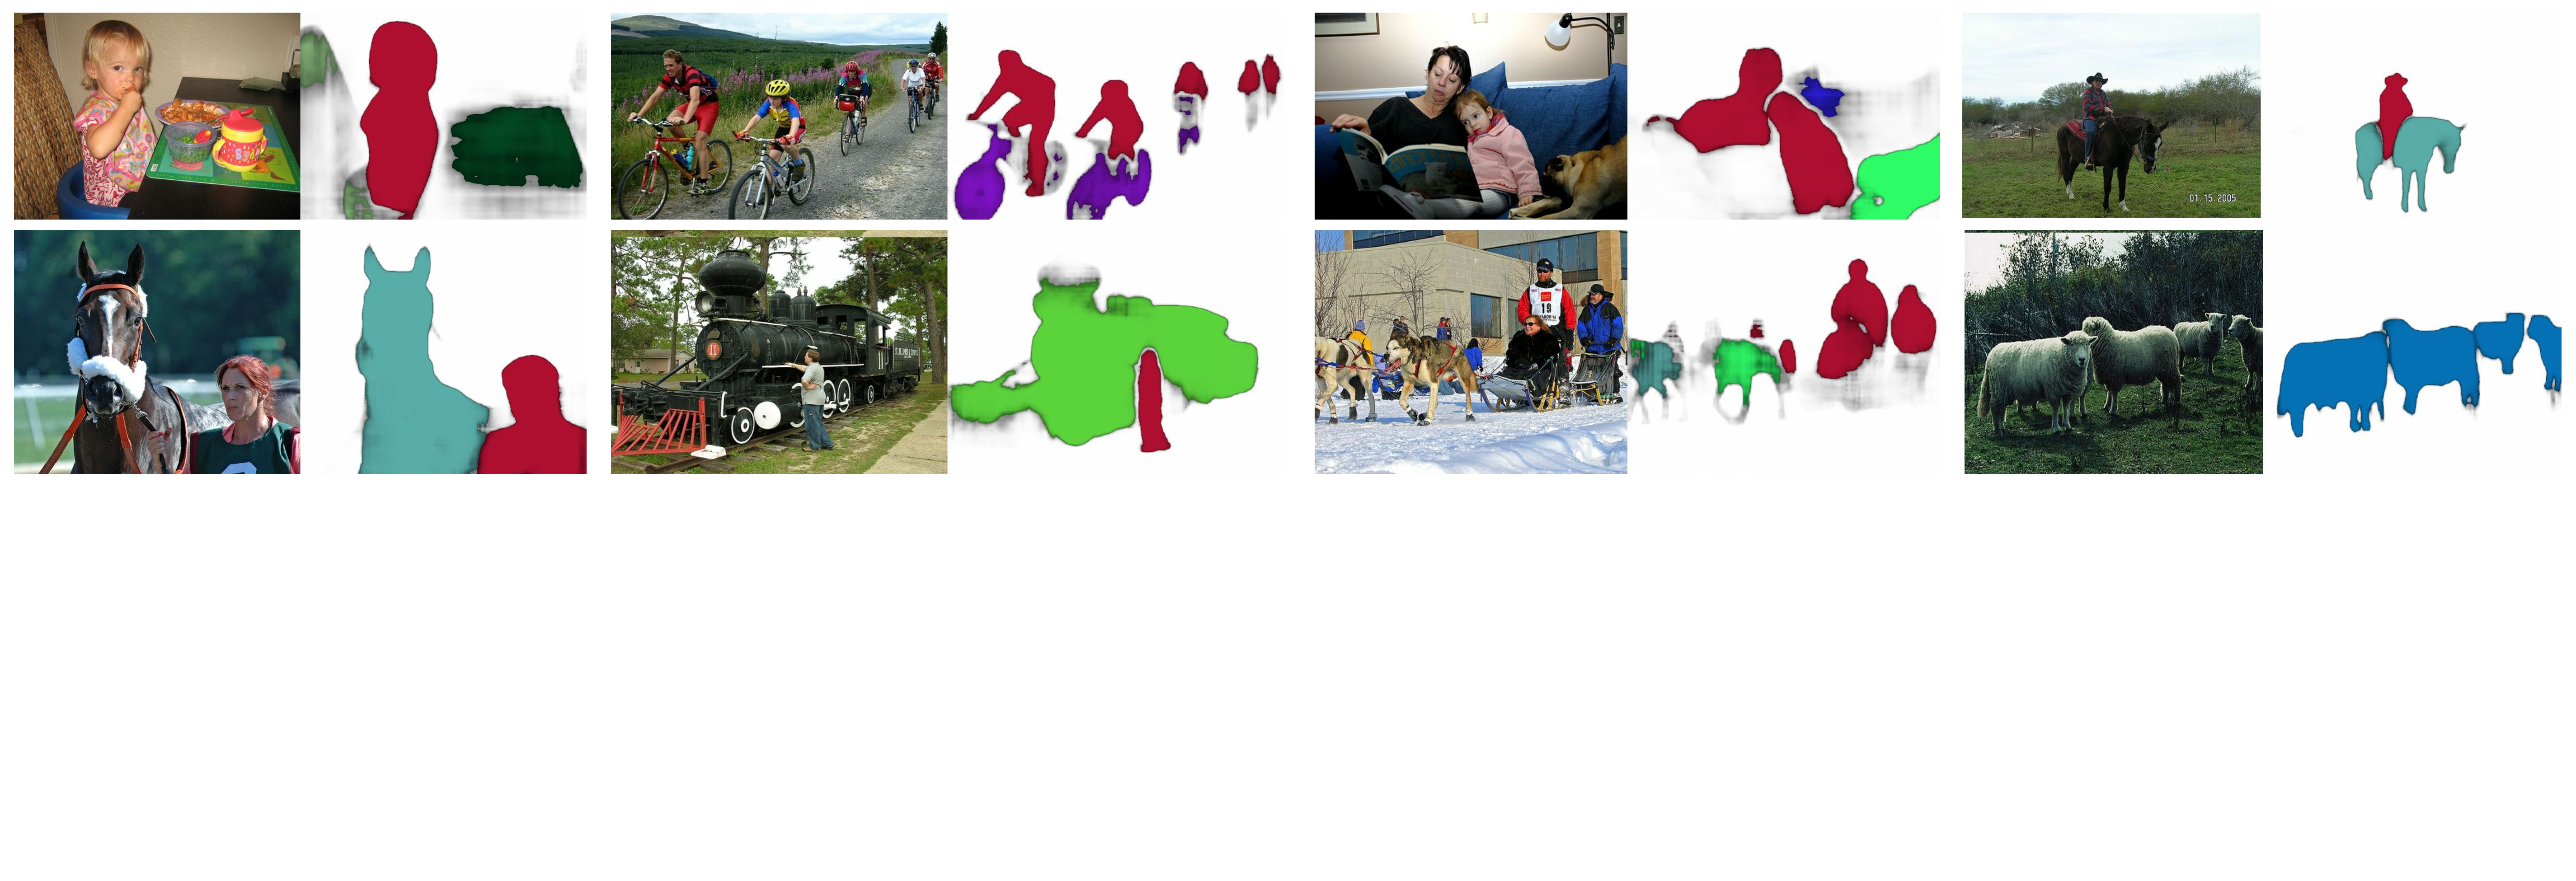
\includegraphics[width=1.\linewidth]{figures/deep_metric_learning/mask_classification.pdf}
  \caption{Deep Metric Learning~\deepml instance segmentation results. }
  \label{fig:deep_metric_learning}
\end{figure}

\section{Video Object Segmentation}
\label{sec:soa:videoobjectsegmentation}

In this section we explore some of the works that tackle object segmentation on videos.

\paragraph{OSVOS~\osvos and OnAVOS~\onavos}
These works focus on instance segmentation on videos.
Their main approach consists of training a parent network that given a frame is able to predict the mask of the foreground (all object instances in the image) and then finetune a network for each video.
The finetuning is performed given the mask of the first frame (these methods tackle semi-supervised video object segmentation) and then the trained network for each video is used to predict the masks for the rest of the frames.
OnAVOS~\onavos extends \osvos by adding an online training step.
It makes predictions of the frames and after each frame prediction, the network is trained online with the new predicted mask.
This two implementations lead to state-of-the-art results on the DAVIS~\davisboth dataset.

\paragraph{MaskRNN~\maskrnn}
This work proposes a recurrent neural network approach which fuses in each frame of the video the output of two deep nets for each objects instance.
The first net is a binary segmentation network providing a mask and the second one is a localization network providing a bounding box.
Thanks to the recurrent component and the localization component, this method is able to take advantage of long-term temporal structures of the video as well as rejecting outliers.
This method also provides competitive results to the works of OSVOS~\osvos and OnAVOS~\onavos presented in the previous subsection.

% \paragraph{Proposal Free Network}~\cite{liang2015proposal}
